\documentclass[11pt,letterpaper]{article}
\usepackage[utf8]{inputenc}
\usepackage[spanish]{babel}\decimalpoint
\usepackage{amsmath}
\usepackage{amsfonts}
\usepackage{amssymb}
\usepackage{physics}
\usepackage{hyperref}
\usepackage[left=2cm,right=2cm,top=2cm,bottom=2cm]{geometry}


\usepackage{graphicx}
\graphicspath{{img_tarea-04/}}
\usepackage{subfig}


\usepackage[draft,inline,nomargin]{fixme} \fxsetup{theme=color}
\definecolor{jacolor}{RGB}{200,40,0} \FXRegisterAuthor{ja}{aja}{\color{jacolor}JA}

\newcommand{\mcM}{\mathcal{M}}

\renewcommand{\labelenumii}{\arabic{enumi}.\arabic{enumii}}
\renewcommand{\labelenumiii}{\arabic{enumi}.\arabic{enumii}.\arabic{enumiii}}
\renewcommand{\labelenumiv}{\arabic{enumi}.\arabic{enumii}.\arabic{enumiii}.\arabic{enumiv}}

\newcommand{\autores}{\text{Baseden y Tye}}


%%%%% Author
\author{José Alfredo de León}

%%%% Title 
\title{Tarea 6: DFT\\
\large{Métodos de Simulación Computacional para Sistemas Cuánticos - 2022-2}}


\begin{document}
\date{08 de abril de 2022}
\maketitle

En este trabajo vamos a reproducir las expresiones y cálculos del funcional
de energía electrónica total para el átomo de Helio de \autores{} en \cite{baseden2014introduction}. 
Para nuestros cálculos tomaremos $\hbar=1$ y $m=1$, así como utilizaremos
unidades atómicas. Es decir, la energía tendrá dimensiones de unidades
de hartree (unidades atómicas).

Resulta útil escribir la energía electrónica total de un átomo o molécula
como
\begin{align}\label{eq:electronic}
E_{tot}=E_T+E_V+E_J+E_X+E_C
\end{align}
donde $E_T$ es la energía cinética total de los electrones, $E_V$ es 
la energía total potencial de los electrones debida a su interacción de 
Coulomb con el centro del núcleo, $E_J$ es la energía potencial total debida al
promedio de repulsión de Coulomb entre pares de electrones, $E_X$ es la energía
cuántica total de intercambio de los electrones y $E_C$ es la energía total
de correlación de los electrones. 

Para representar el orbital $1s$ del átomo de Helio \autores{} utilizan
la aproximación de una función de onda Gaussiana normalizada
\begin{align}\label{psi}
\psi(r)=2\qty(\frac{2\alpha}{\pi})^{3/4}e^{-\alpha r^2}.
\end{align}
Resultados de cálculos más precisos se presentan en \cite{baseden2014introduction}
aproximando la función de onda del orbital $1s$ con una combinación 
lineal de funciones gaussianas. No obstante, la aproximación \eqref{psi}
permite realizar cálculos analíticos.

La idea básica detrás de cálculos como el de Hartree-Fock y el de la teoría 
del funcional de densidad (DFT) es que la energía total electrónica es un
funcional que depende de la función de densida electrónica $n(r)$ como
\begin{align}\label{eq:functional}
E_{tot}[n]=E_T[n]+E_V[n]+E_J[n]+E_X[n]+E_C[n],
\end{align}
donde los términos representan las mismas energías de \eqref{eq:electronic}.
Dicho sea de paso, a diferencia de la función de onda, la densidad 
electrónica es un observable que puede medirse experimentalmente. 

Ahora calculamos los funcionales en \eqref{eq:functional}. Comenzamos
considerando al operador de energía cinética $-1/2\laplacian{}$:
\begin{subequations}\label{T:energy}
\begin{align}
E_T&=\Bigg\langle \psi \Bigg|-\frac{1}{2}\nabla^2\Bigg| \psi \Bigg\rangle\\
&=-\frac{1}{4}\int_0^{2\pi}\int_{0}^{\pi}\int_{0}^{\infty}\psi(r) \qty[-\frac{1}{2}\qty(\frac{2}{r}\frac{d\psi(r)}{r}+\frac{d^2\psi(r)}{r^2})]r^2\sin \theta drd\theta d\phi\\
&=-\pi\int_0^{\infty} \frac{8 \sqrt{2} \alpha ^{5/2} e^{-2 \alpha  r^2} \left(2 \alpha  r^2-3\right)}{\pi ^{3/2}}r^2dr\\
&=\frac{3}{2}\alpha.
\end{align}
\end{subequations}
Ahora calculamos la energía total potencial debida a la interacción de 
Coulomb, considerando que $Z=2$:
\begin{subequations}\label{V:energy}
\begin{align}
E_V&=\Bigg\langle \psi \Bigg|-\frac{2}{r}\Bigg| \psi \Bigg\rangle\\
&=\frac{1}{4}\int_0^{2\pi}\int_{0}^{\pi}\int_{0}^{\infty}\qty(-\frac{2}{r})\frac{8 \sqrt{2} \alpha ^{3/2} e^{-2 \alpha  r^2}}{\pi ^{3/2}} r^2\sin \theta drd\theta d\phi\\
&=-\pi\int_0^{\infty}\frac{16 \sqrt{2} \alpha ^{3/2} r e^{-2 \alpha  r^2}}{\pi ^{3/2}}\  dr\\
&=-3.19154\sqrt{\alpha}.
\end{align}
\end{subequations}
Seguidamente, para calcular 
la expresión para calcular el funcionald de la energía potencial 
debida a la repulsión promedio entre electrones
$E_J[n]$ consideramos la siguiente expresión:
\begin{align}
E_J&=\Big\langle \psi \Big|V_H\Big| \psi \Big\rangle,
\end{align}
donde $V_H$ es el potencial de hartree. Primero debemos
encontrar $V_H$. Para ello, recurrimos a la ecuación de Poisson
\begin{align}
\laplacian{V_H(r)}=-4\pi n(r)
\end{align}
para seguir el programa de Thijssen en \cite{thijssen2007computational}.
Aaprovechamos la simetría radial de 
la densidad electrónica $n(r)$ y definimos $U(r)=rV_H(r)$, la ecuación de Poisson se reduce a
\begin{align}
\frac{d^2 U}{dr^2}&=-4\pi r n(r)=-4\pi r \qty(\frac{\psi(r)}{2})^2\\
\frac{d^2 U}{dr^2}&-\pi r \psi^2(r)
%=-\frac{u^2(r)}{r},\quad u(r)=\sqrt{\pi}r\psi(r),
\end{align}
%donde se está utilizando la condición de normalización
%\begin{align}
%\int r^2\psi(r)dr=1.
%\end{align}
Integrando una vez ambos lados de la ecuación:
\begin{align}
\frac{dU}{dr}= \sqrt{\frac{2\alpha}{\pi }} e^{-2 \alpha  r^2}+c_1,
\end{align}
integrando por segunda vez:
\begin{align}
U(r)=\erf\left(\sqrt{2} \sqrt{\alpha } r\right)+c_1r+c_2,
\end{align}
donde $c_1=0$ y $c_2=0$ para que la función $U(r)$ sea consistente con 
las condiciones de frontera $U(0)=0$ y $U(\infty)=1$. Por consiguiente,
el potencial de hartree se escribe
\begin{align}
V_H(r)=\frac{\erf(r\sqrt{2\alpha})}{r}.
\end{align}
Finalmente calculamos el funcional de energía $E_J$ como
\begin{subequations}\label{J:energy}
\begin{align}
E_J&=\frac{4\pi}{4}\int \psi^*(r)V_H(r)\psi(r)r^2dr\\
&=\frac{4\pi}{\pi}\int_0^{\infty} \psi^2(r)\erf(r\sqrt{2\alpha})rdr\\
&=2\sqrt{\frac{\alpha}{\pi}}
\end{align}
\end{subequations}
Por último, para calcular la energía de intercambio consideramos 
la expresión 
\begin{align}
E_{XC}(\alpha)=-\qty(4\pi)\qty(\frac{3}{4})\qty(\frac{3}{\pi})^{1/3}
\int_0^{\infty} n^{4/3}(r)r^2dr,
\end{align}
donde $n(r)=\frac{1}{2}\psi^2(r)$ y donde se ha introducido una constante
empírica igual a 1.05 de escalamiento que requiere la formulación de Slater,
según \autores{} en \cite{baseden2014introduction}. 
Se sigue entonces 
\begin{subequations}\label{XC:energy}
\begin{align}
E_{XC}(\alpha)&=-(4\pi)\qty(\frac{3}{4})\qty(\frac{3}{\pi})^{1/3}
\int_0^{\infty} \frac{8\cdot 2^{1/3}\alpha^2e^{-\frac{8}{3}\alpha r^2}}{\pi^2}r^2dr,\\
&=-0.9645\sqrt{\alpha}.
\end{align}
\end{subequations}

Ahora, considerando las expresiones de los funcionales en 
\eqref{T:energy}, \eqref{V:energy}, \eqref{J:energy} y \eqref{XC:energy}
podemos escribir los funcionales de energía total siguientes
\begin{enumerate}
\item Sin Hartree-Fock: $E_{tot}=2E_T(\alpha)+2E_V(\alpha)$
\item Con Hartree-Fock: $E_{tot}=2E_T(\alpha)+2E_V(\alpha)+E_J$
\item Con Hartree-Fock más energía de correlaciones: $E_{tot}=2E_T(\alpha)+
2E_V(\alpha)+E_J+\frac{3}{2}E_{XC}$
\end{enumerate}
En la Fig. \ref{fig} mostramos nuestros resultados para la 
energía total electrónica en función del parámetro orbital $\alpha$.

\begin{figure}
%\centering
\hspace{3.2cm}
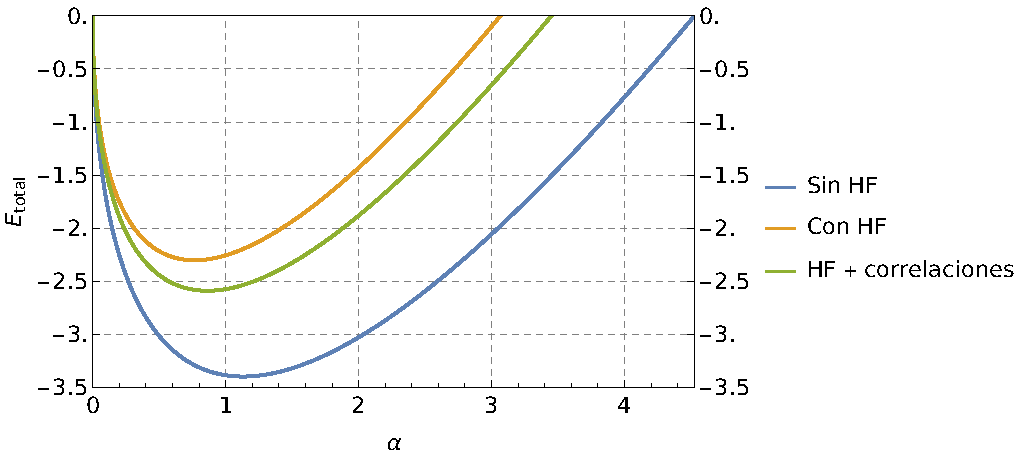
\includegraphics[width=14cm]{fig_tarea06}
\caption{Funcionales de energía electrónica total del átomo de Helio en función
del parámetro de orbital $\alpha$ sin considerar
Hartree-Fock (línea azul), con Hartree-Fock (línea naranja) y con
Hartree-Fock más correlaciones (línea verde).}
\label{fig}
\end{figure}

Para encontrar el valor del parámetro $\alpha$ que minimiza los 
funcionales de energía electrónica total $E_{tot}$ en los diferentes
escenarios resolvemos el problema usual de optimización, es decir, 
encontramos el valor de $\alpha$ para el cual $d E_{tot}=/d\alpha=0$. Para 
el cálculo sin Hartree-Fock encontramos que el parámetro óptimo de orbital es 
$\alpha=1.132$ y un valor mínimo de la energía $E=-3.395$ au. Para 
el funcional de energía con Hartree-Fock se obtiene $\alpha=0.767$ y 
un valor mínimo de energía $E_{tot}=-2.301$ au. Para el funcional de energía 
con Hartree-Fock más correlaciones se obtiene $\alpha=0.0885$ y un valor 
mínimo de la energía $E_{tot}=-2.588$ au.

La mejor aproximación calculada para la energía total electrónica, 
comparada con el valor experimental medido de $-2.9034$ au
\cite{baseden2014introduction},
se obtiene del funcional de energía calculado con Hartree-Fock más 
el término de correlaciones que funciona como corrección al término
simplificado de interacción de Coulomb entre pares de electrones. 
En la Fig. \ref{fig} observamos que considerar la suma individual 
de energías cinética y potencial de cada electrón sobreestima la energía
total electrónica del Helio y que considerar únicamente como término 
extra de la energía la repulsión de Coulomb entre electrones subestima 
el valor experimental de la energía. Por esta razón, se hace evidente
que debe existir un (unos) termino(s) de corrección a la repulsión 
entre electrones, como lo hace considerar además las correlaciones.
 

\bibliographystyle{unsrt}
\bibliography{references}

\end{document}